\chapter{Implementation}
    \label{chap:implementation}

   This chapter will explain my implementation for this project. It will first give an overview of the architecture of the software product. After that, we will present each one of the challenges that have been implemented so far.

    \section{Architecture} 
        \label{sec:architecture}
        
    The central part of the software implementation consists of the Damn Vulnerable Mobile - Inter Component Communication app. This Android app contains all of the educational material needed to understand Android ICC and complete each challenge, encourages the user to learn interactively,  and it provides access to each challenge and to settings to control the challenge or the learning experience. 
    
    The rest of the project consists of a series of Android apps that play the role of either a vulnerable app or a malware. These apps are made to appear to be authentic apps with real-world functionalities, though many of them are nowhere close to full-feature app. Each challenge consists of an authentic scenario of a malware app attacking one of the vulnerable apps through one particular ICC vulnerability.
    
    The DVM-ICC app communicates with the challenge apps through the use of files in order to apply various settings to control the behaviour of the apps. These settings are explained in subsection \ref{subsec:challenge_settings}. Moreover, each pair of vulnerable and malicious apps communicate between each other as a result of the cyber attack, through the medium of Intents. The manner in which this communication takes place will be explained in detail for each challenge in section \ref{}.
    
    \section{DVM-ICC Application}
        \label{sec:home_app}
        
    In this section, I will explore the features of the DVM-ICC Android app. While doing so, I will explain the intended workflow that a user needs to follow and how app provides an educational experience. The follow description applies to the Beginner mode. The app has three different operation modes, which will be fully explained in subsection \ref{subsec:challenge_modes}.
    
    \subsection{Home Menu}
        \label{subsec:home_menu}
        
    \begin{wrapfigure}[15]{r}{0.3\textwidth}
        \centering
        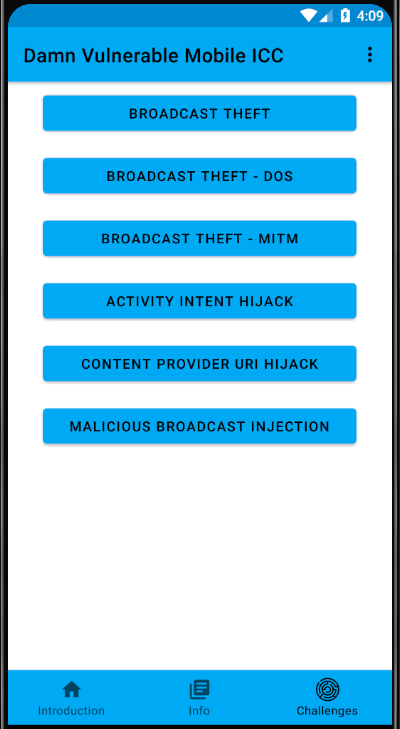
\includegraphics[width=0.3\textwidth]{graphics/home_activity.PNG}
        \caption{The first menu in the DVM-ICC app.}
        \label{fig:home_menu}
    \end{wrapfigure}
        
    The first screen the user sees when starting the app has 3 sub-pages: Introduction, Info and Challenges, as you can see in figure \ref{fig:home_menu}. The Introduction page gives an introduction of the project and explains the intended workflow for using the product. The Info page provides all of the necessary technical background to understand ICC vulnerabilities and attacks. It covers what components and permissions are, how components communicate between each other and the major types of ICC based attacks: Intent Hijacking and Intent Spoofing. The Challenges page lets the user select what challenge they want to start, as shown in figure \ref{fig:home_menu}.
    
    \subsection{Challenge Settings}
        \label{subsec:challenge_settings}
        
    When clicking on a challenge, the user is taken to a menu where they can change the settings that define how the challenge will be undertaken. Here, you can set the operation mode for the challenge. Moreover, the user can enable or disable the malware of the selected challenge. If disabled, the malicious app will not perform any cyber-attack and therefore it will not interfere with any vulnerable app or the rest of the system.
    
    The most important setting on this screen is the security level of the vulnerable app. Inspired from DVWA, as described in subsection \ref{subsec:ICC_related_work}, these levels define how secure the vulnerable app is against attacks from the malware. Each challenge's vulnerable app has between 2 and 5 security levels, with each successive level using more secure code. This culminates with the Impossible level, where the vulnerability is fixed and the malware can not perform the attack. When the malware is enabled, it will overcome the defences of the current security level, except for the Impossible level. The number of security levels and their meaning depends on the challenge. In general, each security level means that a component or broadcast is protected with a more powerful permission, that components are no longer exported or that an intent is now sent explicitly. 
    
    These settings are written to a text file that is located in the DVM-ICC's app specific directory on the device's external storage, from where it can be accessed by any other app, including the other apps that are part of this project. The security level setting will dynamically change the behaviour of the vulnerable and malicious apps, and the user does not need to restart them, with some
    exceptions. The challenge settings can be changed at any time while doing a challenge.
    
    \subsection{Identifying the malware and the vulnerable app}
        \label{subsec:identify_challenge_apps}
        
    \begin{wrapfigure}[19]{r}{0.4\textwidth}
        \centering
        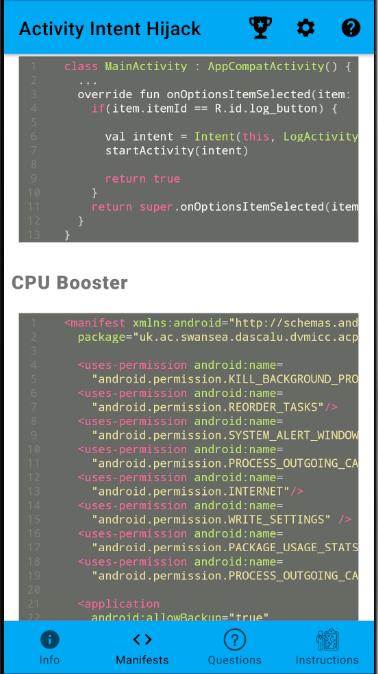
\includegraphics[width=0.4\textwidth]{graphics/manifests.PNG}
        \caption{The Manifests page in the Challenge activity.}
        \label{fig:manifests_fragment}
    \end{wrapfigure}
        
    Once the user applies the settings described in subsection \ref{subsec:challenge_settings}, the application starts the Challenge activity, which you can see in figure \ref{fig:manifests_fragment}. The first task of every challenge is to identify the pair of vulnerable and malicious apps for that challenge from amongst all of the apps that are part of the project, except the DVM-ICC app itself. 
    
    The Info page gives a technical description of one of the two major attack categories, Intent Hijacking or Intent Spoofing, followed by a detailed description of the specific cyber attack related to this challenge. After reading and understanding this information, the user needs to go the Manifests page, where they can view for each app the contents of its manifest and all snippets of code that sends intents, as shown in figure \ref{fig:manifests_fragment}. Based on the technical background the user was given in the Info page and in the Home Menu from subsection \ref{subsec:home_menu}, they need to look through the code in the Manifests page and try to identify the vulnerable app and the malware for this challenge. 
    
    The user should be able to detect vulnerable apps by looking for intents being sent implicitly or for exported components, for example. Malwares can be usually identified by the use of intent filters matching intents that are only sent by a vulnerable app, or by sending an explicit intent to another app that is part of this project. The features that identify the vulnerable app and the malware depend on the selected challenge.
    
    The Questions page contains text boxes where the user can type in their answers and be told if they have correctly identified the apps.
    
    \subsection{Performing the cyber-attack}
        \label{subsec:perform_attack}
        
    Now that the user knows the correct pair of apps for this challenge, the next task of the challenge is to use these apps to witness the cyber-attack take place.
    
    \begin{wrapfigure}[20]{r}{0.4\textwidth}
        \centering
        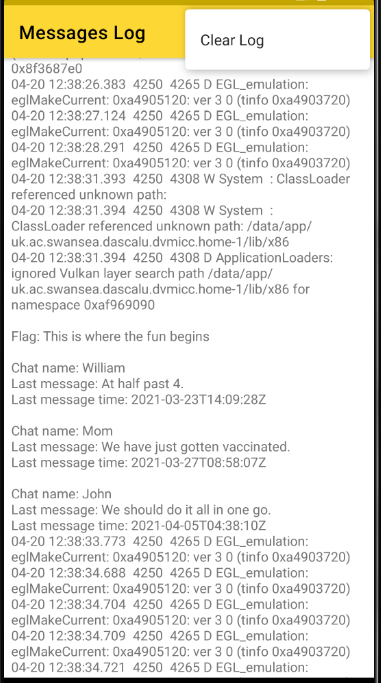
\includegraphics[width=0.4\textwidth]{graphics/log.PNG}
        \caption{Log of the malware for Content Provider URI Hijack after it successfully attacked the vulnerable app.}
        \label{fig:malware_log}
    \end{wrapfigure}
    
    Once you have correctly answered the questions regarding the identity of the malware and vulnerable app, the Instructions page will display detailed instructions for using the apps such that the specific cyber-attack for that challenge will take place. This page can be accessed from the activity shown in figure \ref{fig:manifests_fragment}.
    
    In general, the user is asked to take a look at the two apps to familiarise themselves with them and what they can do. Then, the user should make sure that the security level is set to low. After that, they should use the vulnerable app and malware according to the provided instructions in order to trigger the attack and observe it. 
    
    Following that, the user needs to go the malware and look in its Log, which is accessed from its app bar. If the attack was successful, the malware should have written in its log the flag associated with this specific challenge and security level, along with any relevant data it managed to steal from the vulnerable app. These would be hidden amongst the output of Android Log. 
    
    You can see an example of this in figure \ref{fig:malware_log}, where the messages from the Whatsapp vulnerable app have been stolen by the SMS Messages malware. The user should then copy the flag and submit it to the flag question for the current security level in the Questions page in the DVM-ICC app, to prove they have completed one level of the challenge. 
    
    At this point, the user should clear the log of the malware, to see the effects of the next attack more easily, and then change the security level to the next value. They should repeat the process described in this subsection for every security level of that challenge.
    
    Through performing the task described in this section, the user will witness an example of a cyber attack happening in an authentic scenario, with a real malicious app exploiting an insecure app. 
    
    \subsection{Security Levels Explanation}
        \label{subsec:security_levels_explanation}
        
    \begin{wrapfigure}[22]{r}{0.45\textwidth}
        \centering
        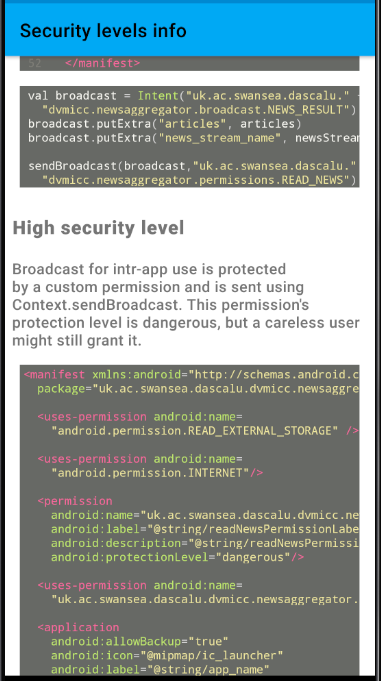
\includegraphics[width=0.45\textwidth]{graphics/security_level_explanation.PNG}
        \caption{Part of the explanation of the security levels for the Broadcast Theft Challenge.}
        \label{fig:security_levels}
    \end{wrapfigure}
        
    While completing the task described in subsection \ref{subsec:perform_attack}, the user can click on the Help button that you can see at the top right in figure \ref{fig:manifests_fragment} to view an explanation of the security levels for the current challenge.
    This view is hidden until the user has identified the pair of apps for the current challenge, as explained in subsection \ref{subsec:identify_challenge_apps}.
    
    For each level, it will explain how it works and how it is more secure than the previous level. Following this explanation is a view of the full manifest of the vulnerable app, as it would be used for that security level. Finally, this view might show code snippets that introduce a vulnerability through the way they send an intent.
        
    You can see part of the Security Levels explanation for the Broadcast Theft challenge in figure \ref{fig:security_levels}, as an example. The top code snippet shows the code used to send a broadcast in the News Aggregator app in the medium security level. Since this code send the broadcast implicitly, it is insecure.
    
    This activity teaches the user how and where the vulnerability is introduced and what steps a programmer can take to secure the vulnerable app, complete with code examples from the app itself. Some solutions fail to completely remove the vulnerability, and this activity teaches the developer why they are inadequate. The explanation of the Impossible level shows how to completely remove the attack surface.
    
    By looking at these explanations while performing the task described in subsection \ref{subsec:perform_attack}, the user will be able to see how the cyber attack of that challenge can still succeed despite the programmer implementing some security defences.
    
    \subsection{Challenge Conclusion}
        \label{subsec:challenge_conclusion}
    
    Once the user has performed the cyber attack and has submitted the correct flag for every security level of the challenge, they have completed that challenge. As a reward, they can now click on the trophy button on the app bar of the Challenge activity, which you can see in figure \ref{fig:manifests_fragment}.
    
    This will open an activity where the user can read the conclusion to the current challenge. This text will give a summary of the whole challenge, going through how the vulnerability is introduced, how the attacker can create a malware that takes advantage of it, and how to fix the vulnerability. Moreover, the conclusion will comment on the authenticity of the scenario presented in the challenge, covering how or why the vulnerability was introduced in the first place and how likely it is for the scenario might to be encountered in the real world. The purpose of this conclusion is condense all of the information that the user should take away from this challenge.
    
    \subsection{Operation Modes}
        \label{subsec:challenge_modes}
    
    As mentioned at the beginning of section \ref{sec:home_app}, the DVM-ICC application supports three modes. The Beginner mode has already been described in sub\cref{subsec:home_menu,subsec:challenge_settings,subsec:identify_challenge_apps,subsec:perform_attack,subsec:security_levels_explanation,subsec:challenge_conclusion}. It is meant for less experienced users, who need to given detailed explanations in order to understand the ICC vulnerabilities of each challenge.
    
    The Expert Mode works in the same way as the Beginner mode, but it hides a lot of information from the user to increase the difficulty. In the Challenge activity from figure \ref{fig:manifests_fragment} on page \pageref{fig:manifests_fragment}, the Info page will be hidden, and the Security Levels Explanation activity from figure \ref{fig:security_levels} will only contain code snippets, without any of the explanations.
    
    The Make your own Malware mode disables the malware app of the current challenge in order to allow the user to create their own malware and attack the vulnerable app without interference from the included malware. In this mode, the user only has access to the Info page described in subsection \ref{subsec:identify_challenge_apps} and the Security Levels activity described in subsection \ref{subsec:security_levels_explanation}.
    